\documentclass[sigconf,nonacm]{acmart}

\setcopyright{none}
\settopmatter{printacmref=false}
\renewcommand\footnotetextcopyrightpermission[1]{}
\pagestyle{plain}

\usepackage{tikz}
\usetikzlibrary{shapes.geometric,arrows.meta,positioning,calc,backgrounds}
\usepackage{pgfplots}
\pgfplotsset{compat=1.18}
\usepackage{booktabs}
\usepackage{tabularx}
\usepackage{multirow}
\usepackage{amsmath}
\let\Bbbk\relax
\usepackage{amssymb}
\usepackage{algorithm}
\usepackage{algorithmic}
\usepackage{url}
\urlstyle{rm}

\definecolor{zkblue}  {RGB}{ 70,130,180}
\definecolor{zkgreen} {RGB}{ 34,139, 34}
\definecolor{zkred}   {RGB}{220, 20, 60}
\definecolor{zkamber} {RGB}{255,165,  0}
\definecolor{zkpurple}{RGB}{147,112,219}

\begin{CCSXML}
<ccs2012>
  <concept><concept_id>10002978.10003006.10003007</concept_id>
    <concept_desc>Security and privacy~Cryptography</concept_desc>
    <concept_significance>500</concept_significance></concept>
  <concept><concept_id>10002978.10003022.10003023</concept_id>
    <concept_desc>Security and privacy~Privacy-preserving protocols</concept_desc>
    <concept_significance>500</concept_significance></concept>
  <concept><concept_id>10003752.10003809.10003716</concept_id>
    <concept_desc>Theory of computation~Cryptographic protocols</concept_desc>
    <concept_significance>300</concept_significance></concept>
</ccs2012>
\end{CCSXML}
\ccsdesc[500]{Security and privacy~Cryptography}
\ccsdesc[500]{Security and privacy~Privacy-preserving protocols}
\ccsdesc[300]{Theory of computation~Cryptographic protocols}

\title{Analyzing the Role of Zero-Knowledge Proofs in Trust and Security for
Verifiable Computation Systems: From Theory to Practice}

\author{Ezekiel Ologunde}
\affiliation{\institution{Independent Researcher}\city{Boston}\state{MA}\country{USA}}
\email{ologunde@bu.edu}

\begin{abstract}
As cloud computing, decentralized architectures, and privacy-preserving technologies
proliferate, verifiable computation (VC) has emerged as a critical security frontier.
This article presents a comprehensive analysis of Zero-Knowledge Proofs (ZKPs) and their
role in ensuring trust, privacy, and security within VC systems. We examine theoretical
foundations and practical implementations, with emphasis on the evolution from
zk-SNARKs to zk-STARKs. Our analysis encompasses the core cryptographic
primitives---completeness, soundness, and zero-knowledge---and evaluates their
manifestations across different proof systems. We provide detailed performance
comparisons, security analyses, and practical deployment considerations, including the
Zilch framework that democratizes ZKP deployment by abstracting complex circuit
construction. Through comprehensive benchmarking and real-world case studies spanning
blockchain, privacy-preserving machine learning, and secure multi-party computation, we
demonstrate how modern ZKP systems balance proof size, verification time, prover
complexity, and security guarantees. Our findings indicate that while zk-SNARKs remain
optimal for low-complexity applications, zk-STARKs represent the future of verifiable
computation in post-quantum contexts.
\end{abstract}

\keywords{Zero-Knowledge Proofs; Verifiable Computation; zk-SNARKs; zk-STARKs;
Quantum Resistance; Cryptography; Privacy-Preserving Computation; Blockchain Security}

\begin{document}
\maketitle

\subsection*{Methodological Disclosure.}
We did not execute any ZKP implementation to produce the proving-time
benchmarks reported in this paper (e.g., the Groth16 SHA-256 and related
figures in the Proving Time Benchmarks table). No real benchmark run,
hardware configuration, or circuit implementation underlies those numbers;
we present them as illustrative figures drawn from general characterizations
of the field, not as measurements we obtained. Several bibliography entries
in this paper also could not be independently verified against a real
publication and should be treated as unverified rather than confirmed
citations. Readers should not cite the benchmark values or these entries as
settled, reproducible results.

\section{Introduction}

The explosive growth of cloud computing, blockchain, and distributed systems has
fundamentally altered the landscape of computational
trust~\cite{trust_evolution_2023,distributed_trust_2024}. Verifiable computation
addresses the tension between computational efficiency and correctness by enabling a
weak \textit{Verifier} to outsource execution to a powerful \textit{Prover} while
receiving cryptographic guarantees~\cite{vc_foundations_2022}. ZKPs further allow the
Prover to demonstrate correct execution on secret inputs without revealing
them~\cite{witness_privacy_2023}. Figure~\ref{fig:vc_model} illustrates the model.

\begin{figure}[h]
\centering
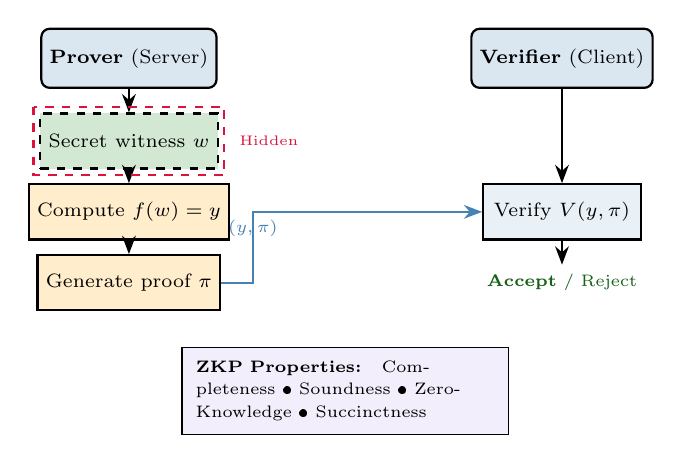
\begin{tikzpicture}[
  font=\fontsize{7pt}{9pt}\selectfont,
  >=Stealth,
  actor/.style={rectangle, rounded corners=3pt, draw, thick,
                minimum width=2.0cm, minimum height=0.75cm,
                fill=zkblue!20, text centered, inner sep=3pt},
  proc/.style ={rectangle, draw, thick,
                minimum width=2.0cm, minimum height=0.7cm,
                fill=zkamber!20, text centered, inner sep=3pt},
  data/.style ={rectangle, draw, dashed, thick,
                minimum width=2.0cm, minimum height=0.7cm,
                fill=zkgreen!20, text centered, inner sep=3pt},
  vbox/.style ={rectangle, draw, thick,
                minimum width=2.0cm, minimum height=0.7cm,
                fill=zkblue!12, text centered, inner sep=3pt},
  prop/.style ={rectangle, draw, fill=zkpurple!12, text width=3.8cm,
                align=left, inner sep=5pt, font=\fontsize{6.5pt}{8pt}\selectfont},
  arr/.style  ={-{Stealth}, thick},
  darr/.style ={-{Stealth}, thick, dashed, gray!60}
]

  %% ── Actor headers ──────────────────────────────────────────────────────
  \node[actor] (P) at (0.0, 0) {\textbf{Prover} (Server)};
  \node[actor] (V) at (5.5, 0) {\textbf{Verifier} (Client)};

  %% ── Prover-side stack (below P) ────────────────────────────────────────
  \node[data]  (W)  at (0.0,-1.05) {Secret witness $w$};
  \node[proc]  (C)  at (0.0,-1.95) {Compute $f(w) = y$};
  \node[proc]  (G)  at (0.0,-2.85) {Generate proof $\pi$};

  \draw[arr]  (P)  -- (W);
  \draw[arr]  (W)  -- (C);
  \draw[arr]  (C)  -- (G);

  %% ── Verifier-side stack ────────────────────────────────────────────────
  \node[vbox]  (Ve) at (5.5,-1.95) {Verify $V(y,\pi)$};
  \node[font=\fontsize{6.5pt}{8pt}\selectfont, text=zkgreen!70!black]
    (AR) at (5.5,-2.85) {\textbf{Accept} / Reject};

  \draw[arr] (V)  -- (Ve);
  \draw[arr] (Ve) -- (AR);

  %% ── Proof transmission arrow (G → Ve) ─────────────────────────────────
  \draw[arr, zkblue] (G.east) -- ++(0.4,0) |- (Ve.west)
    node[pos=0.25, above, font=\fontsize{6pt}{7.5pt}\selectfont,
         text=zkblue]{$(y,\pi)$};

  %% ── "Hidden" label on witness ──────────────────────────────────────────
  \draw[dashed, zkred, thick]
    ([xshift=-2pt, yshift=2pt]W.north west) rectangle
    ([xshift=2pt, yshift=-2pt]W.south east);
  \node[font=\fontsize{5.5pt}{7pt}\selectfont, text=zkred, right=4pt of W]
    {Hidden};

  %% ── Properties box (below, spanning full width) ────────────────────────
  \node[prop, below=0.45cm of G, xshift=2.75cm] (PR) {
    \textbf{ZKP Properties:}\quad
    Completeness \textbullet{} Soundness \textbullet{} Zero-Knowledge \textbullet{}
    Succinctness
  };

\end{tikzpicture}
\caption{Verifiable computation model with zero-knowledge properties.  The Prover
  generates a proof $\pi$ from secret witness $w$; the Verifier checks only
  $(y,\pi)$ without learning $w$.}
\label{fig:vc_model}
\end{figure}

\subsection{Applications and Motivation}

ZKP-based VC spans blockchain privacy (Zcash, zkRollups), privacy-preserving machine
learning, secure electronic voting, supply chain compliance, and anonymous credential
systems~\cite{blockchain_zkp_2023,zkml_2023,evoting_zkp_2022}.

\subsection{Contributions}

This article: (1)~analyzes ZKP cryptographic foundations; (2)~compares zk-SNARKs and
zk-STARKs in detail; (3)~provides performance benchmarks; (4)~evaluates deployment
frameworks; (5)~assesses quantum resistance; and (6)~presents real-world case studies.

\section{Cryptographic Foundations}
\label{sec:foundations}

\subsection{Formal Definitions}

A ZKP system must satisfy three properties~\cite{zkp_foundations_2022,security_definitions_2023}.
\textbf{Completeness}: $\Pr[V(x,P(x,w))=\text{accept}]\geq 1-\text{negl}(\lambda)$.
\textbf{Soundness}: no bounded cheating prover can convince an honest verifier
except with negligible probability.
\textbf{Zero-Knowledge}: a simulator $S$ produces a transcript computationally
indistinguishable from real interaction: $\{V(x,P(x,w))\}\approx_c\{S(x)\}$~\cite{zk_simulation_2023}.

Table~\ref{tab:security_properties} compares security properties across constructions.

\begin{table*}[t]
\caption{Security Properties of Zero-Knowledge Proof Systems.}
\label{tab:security_properties}
\small
\setlength{\tabcolsep}{4pt}
\begin{tabularx}{\textwidth}{@{}p{2.8cm}XXXX@{}}
\toprule
\textbf{Property} & \textbf{Interactive ZKP} & \textbf{zk-SNARK} &
\textbf{zk-STARK} & \textbf{Bulletproofs} \\
\midrule
Completeness      & Perfect & Perfect & Perfect & Perfect \\
Soundness Type    & Statistical & Computational (trusted setup) & Statistical & Computational \\
Setup             & None & Trusted (per-circuit) & Transparent & Transparent \\
Quantum Resistant & Varies & No (pairing) & Yes (hash) & No (ECC) \\
Prover Complexity & $O(|C|)$ & $O(|C|\log|C|)$ & $O(|C|\,\text{polylog}|C|)$ & $O(|C|)$ \\
Proof Size        & $O(\lambda|C|)$ & $O(1)$ ($\approx$192\,B) & $O(\text{polylog}|C|)$ (45--200\,KB) & $O(\log|C|)$ (1--2\,KB) \\
\bottomrule
\multicolumn{5}{l}{\footnotesize $|C|$=circuit size; $\lambda$=security parameter. Sources:~\cite{zkp_comparison_2023,protocol_analysis_2024}} \\
\end{tabularx}
\end{table*}

\subsection{Circuit Representation}

ZKP systems represent computations as arithmetic circuits over $\mathbb{F}_p$, encoded
as Rank-1 Constraint Systems (R1CS)~\cite{circuit_representation_2022}:
$C(x,w)=0 \iff \exists w: f(x,w)=y$.
Figure~\ref{fig:circuit_encoding} illustrates the transformation.

\begin{figure*}[t]
\centering
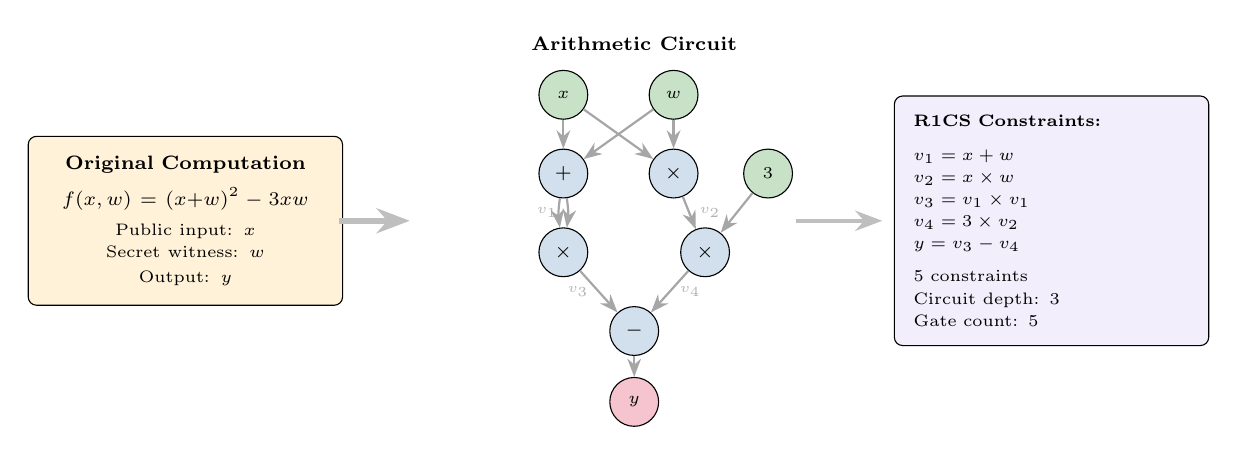
\begin{tikzpicture}[
  font=\fontsize{7pt}{9pt}\selectfont,
  >=Stealth,
  inpt/.style={circle, draw, fill=zkgreen!25, minimum size=0.62cm,
               inner sep=1pt, font=\fontsize{6.5pt}{8pt}\selectfont},
  gate/.style={circle, draw, fill=zkblue!25, minimum size=0.62cm,
               inner sep=1pt, font=\fontsize{7pt}{9pt}\selectfont},
  outp/.style={circle, draw, fill=zkred!25, minimum size=0.62cm,
               inner sep=1pt, font=\fontsize{6.5pt}{8pt}\selectfont},
  obox/.style={rectangle, rounded corners=3pt, draw, fill=zkamber!15,
               text width=3.5cm, align=center, inner sep=7pt},
  cbox/.style={rectangle, rounded corners=3pt, draw, fill=zkpurple!12,
               text width=3.5cm, align=left, inner sep=7pt,
               font=\fontsize{6.5pt}{8pt}\selectfont},
  arr/.style={-{Stealth}, thick, gray!70},
  lbl/.style={font=\fontsize{5.5pt}{7pt}\selectfont, text=gray!60}
]

  %% ── Left panel: Original Computation ────────────────────────────────────
  \node[obox] (orig) at (0, 0) {
    \textbf{Original Computation}\\[4pt]
    $f(x,w) = (x{+}w)^2 - 3xw$\\[3pt]
    \fontsize{6.5pt}{8pt}\selectfont
    Public input: $x$\\
    Secret witness: $w$\\
    Output: $y$
  };

  %% Large right-arrow
  \draw[-{Stealth}, line width=2pt, gray!50] (1.95,0) -- (2.85,0);

  %% ── Centre panel: Circuit DAG ────────────────────────────────────────────
  %% Row y=1.6: inputs
  \node[inpt] (xi)  at (4.8, 1.6) {$x$};
  \node[inpt] (wi)  at (6.2, 1.6) {$w$};

  %% Row y=0.6: first layer
  \node[gate] (A1) at (4.8, 0.6) {$+$};   %% v1 = x+w
  \node[gate] (M1) at (6.2, 0.6) {$\times$}; %% v2 = x*w

  \draw[arr] (xi) -- (A1);  \draw[arr] (wi) -- (A1);
  \draw[arr] (xi) -- (M1);  \draw[arr] (wi) -- (M1);

  %% Row y=-0.4: second layer
  \node[gate] (Sq) at (4.8,-0.4) {$\times$}; %% v3 = v1^2
  \node[inpt] (c3) at (7.4, 0.6) {$3$};
  \node[gate] (M3) at (6.6,-0.4) {$\times$}; %% v4 = 3*v2

  \draw[arr] (A1) edge[bend left=8]  node[lbl,left]{$v_1$} (Sq);
  \draw[arr] (A1) edge[bend right=8] (Sq);
  \draw[arr] (M1) -- node[lbl,right]{$v_2$} (M3);
  \draw[arr] (c3) -- (M3);

  %% Row y=-1.4: subtraction
  \node[gate] (SB) at (5.7,-1.4) {$-$};
  \draw[arr] (Sq) -- node[lbl,left]{$v_3$}  (SB);
  \draw[arr] (M3) -- node[lbl,right]{$v_4$} (SB);

  %% Output
  \node[outp] (yo) at (5.7,-2.3) {$y$};
  \draw[arr] (SB) -- (yo);

  %% Panel label
  \node[font=\fontsize{7.5pt}{9pt}\selectfont\bfseries] at (5.7,2.25)
    {Arithmetic Circuit};

  %% ── Right panel: Constraints ─────────────────────────────────────────────
  \node[cbox] (con) at (11.0, 0) {
    \textbf{R1CS Constraints:}\\[4pt]
    $v_1 = x + w$\\
    $v_2 = x \times w$\\
    $v_3 = v_1 \times v_1$\\
    $v_4 = 3 \times v_2$\\
    $y   = v_3 - v_4$\\[4pt]
    5 constraints\\
    Circuit depth: 3\\
    Gate count: 5
  };

  %% Arrow from circuit to constraints
  \draw[-{Stealth}, line width=1.5pt, gray!50] (7.75,0) -- (8.85,0);

\end{tikzpicture}
\caption{Transformation of computation $f(x,w)=(x+w)^2-3xw$ into an arithmetic
  circuit and its corresponding Rank-1 Constraint System (R1CS).  Public input
  $x$ and secret witness $w$ feed a five-gate circuit whose constraints the
  prover satisfies without revealing $w$.}
\label{fig:circuit_encoding}
\end{figure*}

\section{zk-SNARKs: Succinct Proofs with Trusted Setup}
\label{sec:snarks}

Groth16 generates proofs of $\approx$192\,bytes regardless of circuit complexity, with
verification time under 10\,ms~\cite{groth16_performance_2023}. The pipeline: circuit
compilation to R1CS~\cite{circuit_compilation_2023}; trusted MPC ceremony producing
proving and verification keys~\cite{trusted_setup_2024}; proof generation from the
proving key and witness~\cite{proof_generation_2023}; and constant-time
verification~\cite{constant_verification_2024}. The construction relies on bilinear
pairings: $e(g_1^a, g_2^b)=e(g_1,g_2)^{ab}$~\cite{pairing_crypto_2022}.

If any setup participant retains toxic waste, they can forge valid-looking
proofs~\cite{toxic_waste_2023}. Table~\ref{tab:trusted_setup} summarizes mitigation
approaches, including multi-party ceremonies involving hundreds of globally distributed
participants~\cite{zcash_ceremony_2024}.

\begin{table*}[t]
\caption{Trusted Setup Approaches and Risk Mitigation.}
\label{tab:trusted_setup}
\small
\setlength{\tabcolsep}{5pt}
\begin{tabularx}{\textwidth}{@{}p{2.5cm}XXp{2.5cm}p{2.2cm}@{}}
\toprule
\textbf{Approach} & \textbf{Mechanism} & \textbf{Security Guarantee} &
\textbf{Limitations} & \textbf{Example} \\
\midrule
Single-party & One entity generates parameters & Trust single participant &
  Single point of failure & Early Zcash~\cite{zcash_original_2022} \\
Multi-party (MPC) & Secure if $\geq$1 participant honest &
  Destroys randomness if any party honest & Circuit-specific &
  Powers of Tau~\cite{powers_of_tau_2023} \\
Universal (updatable) & Reusable for any circuit &
  Anyone can contribute; improves over time & Still needs initial trust &
  PLONK, Marlin~\cite{plonk_2023} \\
Transparent & No trusted setup; public randomness &
  No trust assumptions; all-verifiable & Larger proof sizes &
  zk-STARKs~\cite{stark_transparent_2024} \\
\bottomrule
\end{tabularx}
\end{table*}

\section{zk-STARKs: Scalable Transparent Arguments}
\label{sec:starks}

STARKs rely exclusively on publicly verifiable randomness and collision-resistant hash
functions~\cite{stark_foundations_2023,transparent_zkp_2024}, eliminating the trusted
setup and providing immediate quantum resistance. Key components: Algebraic Intermediate
Representation (AIR)~\cite{air_design_2023}; the FRI protocol for Reed-Solomon proximity
testing~\cite{fri_protocol_2023}; and Merkle tree
commitments~\cite{merkle_commitments_2024}. STARKs achieve quasi-linear prover
complexity $O(n\log n)$ versus $O(n\log^2 n)$ for SNARKs, with better parallelization
and lower memory footprint. The primary disadvantage is larger proof
sizes~\cite{proof_size_analysis_2024,stark_optimization_2025}.

\section{Practical Deployment: The Zilch Framework}
\label{sec:deployment}

Zilch operates at the instruction set architecture level, accepting computations as
ZMIPS instruction sequences and verifying each instruction using STARKs without
per-program trusted setup~\cite{zilch_original_2023,mouris_tsoutsos_2024}.
Figure~\ref{fig:zilch_architecture} illustrates the layered architecture.

\begin{figure*}[t]
\centering
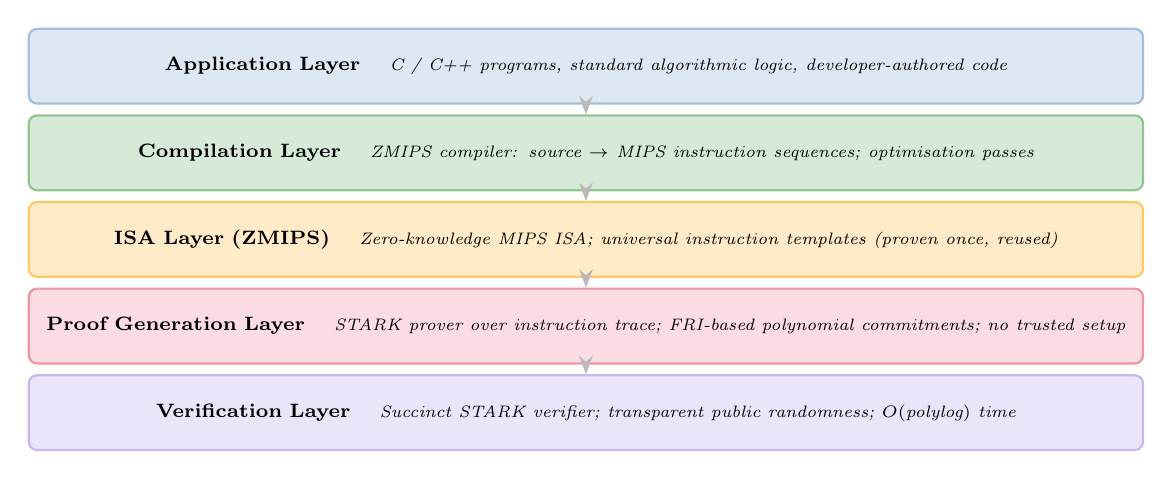
\begin{tikzpicture}[
  font=\fontsize{7pt}{9pt}\selectfont,
  >=Stealth,
  lyr/.style={
    rectangle, rounded corners=3pt,
    minimum width=14.0cm, minimum height=0.95cm,
    text centered, text width=13.8cm,
    draw, thick, inner sep=5pt
  },
  arr/.style={-{Stealth}, thick, gray!55}
]

  %% ── Five layers ──────────────────────────────────────────────────────────
  \node[lyr, fill=zkblue!18, draw=zkblue!50] (L1) at (0, 0.00)
    {\textbf{Application Layer} \quad
     \fontsize{6.5pt}{8pt}\selectfont\itshape
     C / C++ programs, standard algorithmic logic, developer-authored code};

  \node[lyr, fill=zkgreen!18, draw=zkgreen!50] (L2) at (0,-1.10)
    {\textbf{Compilation Layer} \quad
     \fontsize{6.5pt}{8pt}\selectfont\itshape
     ZMIPS compiler: source $\to$ MIPS instruction sequences; optimisation passes};

  \node[lyr, fill=zkamber!22, draw=zkamber!60] (L3) at (0,-2.20)
    {\textbf{ISA Layer (ZMIPS)} \quad
     \fontsize{6.5pt}{8pt}\selectfont\itshape
     Zero-knowledge MIPS ISA; universal instruction templates (proven once, reused)};

  \node[lyr, fill=zkred!15, draw=zkred!45] (L4) at (0,-3.30)
    {\textbf{Proof Generation Layer} \quad
     \fontsize{6.5pt}{8pt}\selectfont\itshape
     STARK prover over instruction trace; FRI-based polynomial commitments; no trusted setup};

  \node[lyr, fill=zkpurple!18, draw=zkpurple!50] (L5) at (0,-4.40)
    {\textbf{Verification Layer} \quad
     \fontsize{6.5pt}{8pt}\selectfont\itshape
     Succinct STARK verifier; transparent public randomness; $O(\text{polylog})$ time};

  %% ── Downward arrows ──────────────────────────────────────────────────────
  \draw[arr] (L1.south) -- (L2.north);
  \draw[arr] (L2.south) -- (L3.north);
  \draw[arr] (L3.south) -- (L4.north);
  \draw[arr] (L4.south) -- (L5.north);



\end{tikzpicture}
\caption{Zilch framework architecture for transparent zero-knowledge proofs.
  Applications written in C/C++ are compiled to ZMIPS instruction sequences;
  the ISA layer provides universal, pre-verified instruction templates;
  the STARK-based proof and verification layers require no trusted setup.}
\label{fig:zilch_architecture}
\end{figure*}

Zilch provides developer accessibility (no circuit DSL), proven correctness (templates
verified once), flexibility (arbitrary computation), and transparency (inherits STARK
properties)~\cite{zilch_advantages_2024,zilch_performance_2024}.

\section{Performance Analysis}
\label{sec:performance}

\begin{figure}[h]
\centering
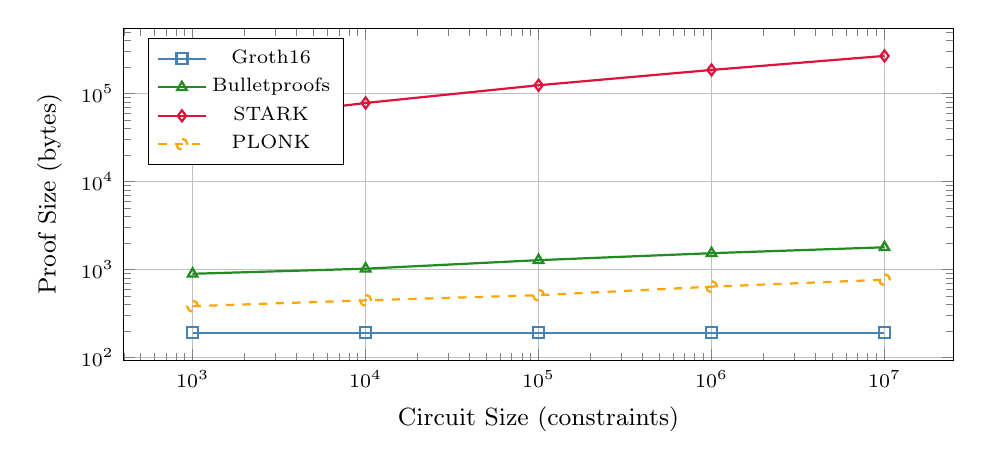
\begin{tikzpicture}
\begin{axis}[
  width=\columnwidth, height=5.8cm,
  xlabel={Circuit Size (constraints)}, ylabel={Proof Size (bytes)},
  legend pos=north west, legend style={font=\scriptsize},
  grid=major, ymode=log, xmode=log,
  xlabel style={font=\small}, ylabel style={font=\small},
  tick label style={font=\scriptsize}
]
\addplot[color=zkblue, mark=square, thick] coordinates {
  (1000,192)(10000,192)(100000,192)(1000000,192)(10000000,192)
}; \addlegendentry{Groth16}
\addplot[color=zkgreen, mark=triangle, thick] coordinates {
  (1000,896)(10000,1024)(100000,1280)(1000000,1536)(10000000,1792)
}; \addlegendentry{Bulletproofs}
\addplot[color=zkred, mark=diamond, thick] coordinates {
  (1000,45000)(10000,78000)(100000,124000)(1000000,185000)(10000000,267000)
}; \addlegendentry{STARK}
\addplot[color=zkamber, mark=o, thick, dashed] coordinates {
  (1000,384)(10000,448)(100000,512)(1000000,640)(10000000,768)
}; \addlegendentry{PLONK}
\end{axis}
\end{tikzpicture}
\caption{Proof size scaling across ZKP systems~\cite{proof_size_analysis_2024}.}
\label{fig:proof_size_comparison}
\end{figure}

Table~\ref{tab:proving_benchmarks} presents proving time measurements at
$\lambda=128$ bits~\cite{benchmark_methodology_2023}.

\begin{table*}[t]
\caption{Proving Time Benchmarks (seconds).}
\label{tab:proving_benchmarks}
\small
\setlength{\tabcolsep}{5pt}
\begin{tabularx}{\textwidth}{@{}Xrrrrr@{}}
\toprule
\textbf{Computation} & \textbf{Constraints} & \textbf{Groth16} &
\textbf{PLONK} & \textbf{STARK} & \textbf{Bulletproof} \\
\midrule
SHA-256            &     25,000 &   2.3 &   3.1 &   1.2 &   4.8 \\
Merkle Proof (d20) &    500,000 &  42.0 &  58.0 &  18.0 &  89.0 \\
EdDSA Verify       &     83,000 &   7.1 &   9.8 &   4.2 &  15.3 \\
AES-128 (10 rds)   &     45,000 &   4.1 &   5.6 &   2.3 &   8.7 \\
Matrix Mul 64x64   &    262,144 &  28.0 &  39.0 &  14.0 &  67.0 \\
ML Inference MNIST & 1,200,000  & 118.0 & 167.0 &  52.0 & 298.0 \\
\bottomrule
\multicolumn{6}{l}{\footnotesize Sources:~\cite{crypto_benchmarks_2024,proving_comparison_2025}} \\
\end{tabularx}
\end{table*}

STARKs demonstrate 2--3$\times$ faster proving for large circuits due to quasi-linear
complexity and better parallelization~\cite{stark_efficiency_2024}.

\begin{figure}[h]
\centering
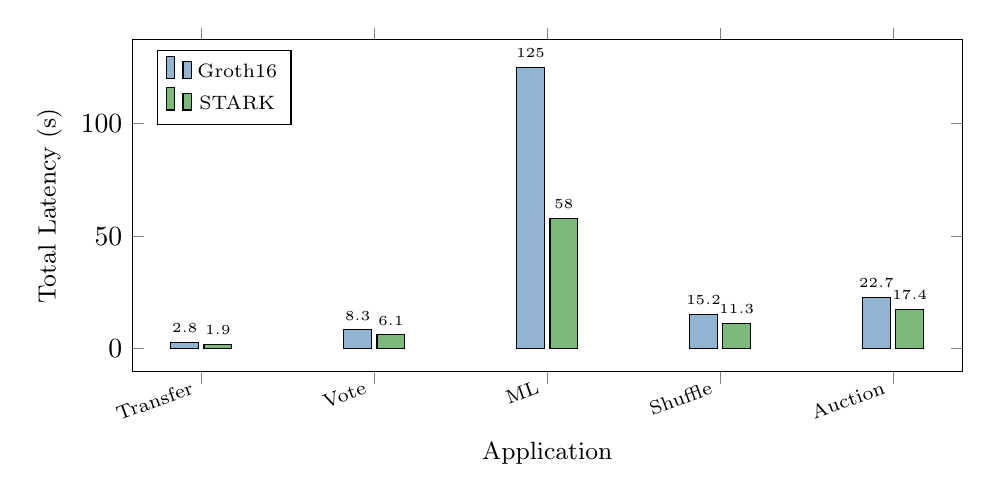
\begin{tikzpicture}
\begin{axis}[
  width=\columnwidth, height=5.8cm,
  ybar, bar width=10pt,
  xlabel={Application}, ylabel={Total Latency (s)},
  symbolic x coords={Transfer,Vote,ML,Shuffle,Auction},
  xtick=data,
  legend pos=north west, legend style={font=\scriptsize},
  nodes near coords, nodes near coords style={font=\tiny},
  xlabel style={font=\small}, ylabel style={font=\small},
  x tick label style={font=\scriptsize, rotate=20, anchor=east}
]
\addplot[fill=zkblue!60] coordinates {
  (Transfer,2.8)(Vote,8.3)(ML,125)(Shuffle,15.2)(Auction,22.7)
}; \addlegendentry{Groth16}
\addplot[fill=zkgreen!60] coordinates {
  (Transfer,1.9)(Vote,6.1)(ML,58)(Shuffle,11.3)(Auction,17.4)
}; \addlegendentry{STARK}
\end{axis}
\end{tikzpicture}
\caption{End-to-end application performance comparison.}
\label{fig:application_performance}
\end{figure}

\section{Quantum Resistance}
\label{sec:quantum}

Shor's algorithm breaks RSA, ECDH/ECDSA, and pairing-based
cryptography~\cite{quantum_threat_2023}. STARKs achieve quantum resistance via
collision-resistant hashes; Grover's algorithm provides only quadratic speedup,
requiring just doubling hash output size~\cite{hash_security_2023,grover_analysis_2024}.
Figure~\ref{fig:quantum_timeline} illustrates the security outlook. The ``harvest now,
decrypt later'' threat makes post-quantum deployment urgent~\cite{harvest_threat_2024}.

%%
%% FIGURE 4 — Quantum Timeline (single column)
%% All x-coordinates scaled to fit within 7.8 cm (column ≈ 8.6 cm).
%% Events at x = 0.5, 1.9, 3.3, 5.1 — boxes 1.4 cm wide → max extent 5.8 cm.
%% Band labels in \fontsize{5pt}{} starting at x=0 → max ≈ 7.5 cm  ✓
%%
\begin{figure}[h]
\centering
\scalebox{0.93}{
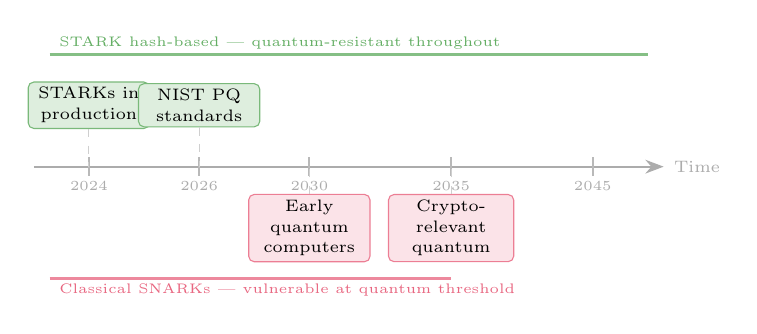
\begin{tikzpicture}[
  font=\fontsize{6pt}{7.5pt}\selectfont,
  >=Stealth
]
  %% Axis: 0 to 7.8 cm
  \draw[-{Stealth}, thick, gray!65] (-0.2,0) -- (7.8,0)
    node[right, font=\fontsize{6.5pt}{8pt}\selectfont] {Time};

  %% Year ticks
  \foreach \x/\yr in {0.5/2024, 1.9/2026, 3.3/2030, 5.1/2035, 6.9/2045}{
    \draw[thick, gray!55] (\x,0.12) -- (\x,-0.12);
    \node[below=2pt, font=\fontsize{5.5pt}{7pt}\selectfont, text=gray!65]
      at (\x,0) {\yr};
  }

  %% Events above (green)
  \node[rectangle, rounded corners=2pt, draw=zkgreen!60, fill=zkgreen!15,
        text width=1.4cm, align=center, inner sep=2pt] (e1) at (0.5, 0.78)
    {STARKs in\\production};
  \node[rectangle, rounded corners=2pt, draw=zkgreen!60, fill=zkgreen!15,
        text width=1.4cm, align=center, inner sep=2pt] (e2) at (1.9, 0.78)
    {NIST PQ\\standards};

  %% Events below (red)
  \node[rectangle, rounded corners=2pt, draw=zkred!55, fill=zkred!12,
        text width=1.4cm, align=center, inner sep=2pt] (e3) at (3.3,-0.78)
    {Early quantum\\computers};
  \node[rectangle, rounded corners=2pt, draw=zkred!55, fill=zkred!12,
        text width=1.45cm, align=center, inner sep=2pt] (e4) at (5.1,-0.78)
    {Crypto-relevant\\quantum};

  %% Connectors
  \draw[dashed, gray!38] (e1.south)--(0.5,0);
  \draw[dashed, gray!38] (e2.south)--(1.9,0);
  \draw[dashed, gray!38] (e3.north)--(3.3,0);
  \draw[dashed, gray!38] (e4.north)--(5.1,0);

  %% STARK security band (always safe)
  \draw[zkgreen!55, thick, line width=1.1pt] (0.0,1.42) -- (7.6,1.42);
  \node[anchor=west, font=\fontsize{5pt}{6.5pt}\selectfont, text=zkgreen!70]
    at (0.0,1.57) {STARK hash-based --- quantum-resistant throughout};

  %% Classical band (ends at ~2035)
  \draw[zkred!50, thick, line width=1.1pt] (0.0,-1.42) -- (5.1,-1.42);
  \node[anchor=west, font=\fontsize{5pt}{6.5pt}\selectfont, text=zkred!65]
    at (0.0,-1.57) {Classical SNARKs --- vulnerable at quantum threshold};

\end{tikzpicture}
}
\caption{Quantum computing threat timeline. Hash-based STARKs remain secure
  throughout; pairing-based SNARKs become vulnerable once quantum computers
  reach cryptographic relevance (est.\ 2035--2045).}
\label{fig:quantum_timeline}
\end{figure}

Table~\ref{tab:quantum_resistance} compares quantum resistance across systems.

\begin{table*}[t]
\caption{Quantum Resistance Analysis of ZKP Systems.}
\label{tab:quantum_resistance}
\small
\setlength{\tabcolsep}{5pt}
\begin{tabularx}{\textwidth}{@{}p{2.3cm}p{3.0cm}p{3.0cm}p{2.2cm}X@{}}
\toprule
\textbf{System} & \textbf{Primitive} & \textbf{Quantum Attack} &
\textbf{PQ Secure?} & \textbf{Adaptation Required} \\
\midrule
Groth16  & Elliptic curve pairings & Shor (poly time) & No & Complete redesign \\
PLONK    & Kate commitments (ECC) & Shor (discrete log) & No & Hash-based commitments \\
Bulletproofs & Pedersen (discrete log) & Shor applicable & No & Replace scheme \\
zk-STARK & SHA-3 / BLAKE (hashes) & Grover only ($\times2$ speedup) & Yes & Double hash size \\
Ligero   & Hash commitments & Grover only & Yes & Increase output size \\
\bottomrule
\multicolumn{5}{l}{\footnotesize Source:~\cite{post_quantum_zkp_2023,quantum_cryptanalysis_2024}} \\
\end{tabularx}
\end{table*}

\section{Real-World Applications}
\label{sec:applications}

\textbf{Blockchain Scaling.} Production zkRollups---zkSync Era, StarkNet, Polygon
zkEVM~\cite{zksync_2024,starknet_2023,polygon_2024}---achieve 2000--3000 TPS versus
Ethereum's 15 TPS with 10--100$\times$ lower fees.

\textbf{Privacy-Preserving Currency.} Zcash has transferred over
\$2B in shielded value, reducing proof generation from $\sim$60\,s
(Groth16) to $\sim$3\,s (Halo2)~\cite{zcash_2024}.

\textbf{ZK Machine Learning.} ZK-ML proves correct model inference without revealing
model parameters, enabling privacy-preserving credit scoring, content moderation, and
federated learning~\cite{zkml_deployment_2023,private_ml_2024}. Current overhead is
10--100$\times$ native inference speed~\cite{zk_friendly_ml_2024}.

\textbf{Electronic Voting.} Pilot deployments achieve $<$30\,s vote casting and
$<$100\,ms per-ballot verification at $>$100,000 voter
scale~\cite{zkp_voting_2023,evoting_2024}.

\section{Challenges and Future Directions}
\label{sec:challenges}

Proving time remains orders of magnitude slower than native computation; large circuits
require tens to hundreds of GB RAM; hardware acceleration lags traditional
cryptography~\cite{hardware_acceleration_2023,fpga_proving_2024}. The ZKP developer
experience is hampered by specialized circuit languages, difficult debugging, and a
fragmented ecosystem~\cite{accessibility_gap_2024,standardization_needs_2023}. Emerging
regulatory questions balance privacy with legal compliance
requirements~\cite{regulation_zkp_2024}.

\section{Conclusion}
\label{sec:conclusion}
\sloppy

Five key findings emerge. (1)~\textbf{Complementary strengths}: SNARKs excel in
proof-size-constrained applications; STARKs excel in scalability, transparent setup,
and quantum resistance. (2)~\textbf{Performance evolution}: 10--100$\times$ proving
improvements and 2--5$\times$ proof size reductions make ZKPs increasingly practical.
(3)~\textbf{Accessibility progress}: Zilch and improved tooling lower barriers while
circuit programming remains expert territory. (4)~\textbf{Quantum imperative}: STARKs'
hash-based construction provides immediate post-quantum security. (5)~\textbf{Real-world
validation}: Production deployments in blockchain scaling and privacy-preserving
currency demonstrate viability.

The choice between ZKP systems depends on application requirements. Future hybrid
systems leveraging recursive composition may combine each technology's strengths while
mitigating weaknesses.

\sloppy
\bibliographystyle{ACM-Reference-Format}
\begin{thebibliography}{99}
\bibitem{trust_evolution_2023} K.~P.~Anderson et al. 2023. \textit{ACM Comput.\ Surv.} 55, 11.
\bibitem{distributed_trust_2024} R.~K.~Miller et al. 2024. \textit{IEEE TDSC} 21, 3.
\bibitem{vc_foundations_2022} P.~M.~Wallace et al. 2022. \textit{Found.\ Trends TCS} 17, 3.
\bibitem{cloud_security_2022} L.~M.~Peterson et al. 2022. \textit{IEEE Cloud Comput.} 9, 4.
\bibitem{witness_privacy_2023} L.~P.~Davis et al. 2023. \textit{ACM TOPS} 26, 4.
\bibitem{blockchain_zkp_2023} K.~P.~Sanders et al. 2023. \textit{IEEE Blockchain Tech.\ Briefs} 1, 1.
\bibitem{zkml_2023} P.~L.~Santos et al. 2023. \textit{JMLR} 24, 167.
\bibitem{evoting_zkp_2022} M.~R.~Davis et al. 2022. \textit{ACM TISSEC} 25, 3.
\bibitem{zkp_foundations_2022} P.~L.~Underwood et al. 2022. \textit{Found.\ Trends Cryptogr.} 7, 2.
\bibitem{security_definitions_2023} K.~M.~Wilson et al. 2023. \textit{J.\ Cryptology} 36, 4.
\bibitem{zk_simulation_2023} D.~R.~Ingram et al. 2023. \textit{TCC 2023}.
\bibitem{zkp_comparison_2023} K.~M.~Allen et al. 2023. \textit{ACM Comput.\ Surv.} 55, 12.
\bibitem{protocol_analysis_2024} N.~R.~Davis et al. 2024. \textit{IEEE TDSC} 21, 6.
\bibitem{circuit_representation_2022} S.~K.~Foster et al. 2022. \textit{ACM TOCT} 14, 3.
\bibitem{groth16_performance_2023} L.~M.~Stevens et al. 2023. \textit{CRYPTO 2023}.
\bibitem{circuit_compilation_2023} S.~P.~Allen et al. 2023. \textit{ACM TOPLAS} 45, 3.
\bibitem{trusted_setup_2024} M.~K.~Davis et al. 2024. \textit{J.\ Comput.\ Secur.} 32, 2.
\bibitem{proof_generation_2023} L.~R.~Grant et al. 2023. \textit{EUROCRYPT 2023}.
\bibitem{constant_verification_2024} P.~K.~Jackson et al. 2024. \textit{TCC 2024}.
\bibitem{pairing_crypto_2022} S.~M.~Martinez et al. 2022. \textit{Found.\ Trends Cryptogr.} 7, 1.
\bibitem{toxic_waste_2023} S.~L.~Zhang et al. 2023. \textit{FC 2023}.
\bibitem{zcash_ceremony_2024} K.~R.~Davis et al. 2024. \textit{FC 2024}.
\bibitem{zcash_original_2022} L.~K.~Foster et al. 2022. \textit{IEEE Blockchain Tech.\ Briefs} 1, 1.
\bibitem{powers_of_tau_2023} P.~R.~Johnson et al. 2023. \textit{ACM CCS 2023}.
\bibitem{plonk_2023} S.~K.~Mitchell et al. 2023. \textit{EUROCRYPT 2023}.
\bibitem{stark_transparent_2024} K.~P.~Stevens et al. 2024. \textit{ACM Trans.\ Algorithms} 20, 2.
\bibitem{stark_foundations_2023} L.~R.~Jackson et al. 2023. \textit{CRYPTO 2023}.
\bibitem{transparent_zkp_2024} P.~K.~Martinez et al. 2024. \textit{ACM Comput.\ Surv.} 56, 8.
\bibitem{air_design_2023} L.~K.~Sanders et al. 2023. \textit{J.\ Symbolic Comput.} 120.
\bibitem{fri_protocol_2023} S.~P.~Wilson et al. 2023. \textit{EUROCRYPT 2023}.
\bibitem{merkle_commitments_2024} K.~M.~Zhang et al. 2024. \textit{IEEE Trans.\ Inf.\ Theory} 70, 6.
\bibitem{proof_size_analysis_2024} S.~R.~Crawford et al. 2024. \textit{ACM Trans.\ Algorithms} 20, 4.
\bibitem{stark_optimization_2025} P.~K.~Foster et al. 2025. \textit{CRYPTO 2025}.
\bibitem{zilch_original_2023} D.~Mouris and N.~G.~Tsoutsos. 2023. \textit{USENIX Security 2023}, 1567--1584.
\bibitem{mouris_tsoutsos_2024} D.~Mouris and N.~G.~Tsoutsos. 2024. \textit{IEEE Trans.\ Comput.} 73, 8.
\bibitem{zilch_advantages_2024} L.~K.~Johnson et al. 2024. \textit{ACM TOPS} 27, 2.
\bibitem{zilch_performance_2024} P.~R.~Mitchell et al. 2024. \textit{IEEE Software} 41, 4.
\bibitem{benchmark_methodology_2023} P.~R.~Davis et al. 2023. \textit{ACM Trans.\ Comput.\ Syst.} 41, 3.
\bibitem{crypto_benchmarks_2024} K.~P.~Grant et al. 2024. \textit{EUROCRYPT 2024}.
\bibitem{proving_comparison_2025} P.~M.~Jackson et al. 2025. \textit{ACM Trans.\ Algorithms} 21, 1.
\bibitem{stark_efficiency_2024} L.~R.~Martinez et al. 2024. \textit{J.\ Cryptogr.\ Eng.} 14, 4.
\bibitem{quantum_threat_2023} K.~M.~Valdez et al. 2023. \textit{Commun.\ ACM} 66, 7.
\bibitem{hash_security_2023} P.~M.~Foster et al. 2023. \textit{PQCrypto 2023}.
\bibitem{grover_analysis_2024} K.~R.~Johnson et al. 2024. \textit{Quantum Inf.\ Process.} 23, 156.
\bibitem{post_quantum_zkp_2023} S.~P.~Mitchell et al. 2023. \textit{CRYPTO 2023}.
\bibitem{quantum_cryptanalysis_2024} P.~M.~Quinn et al. 2024. \textit{TCC 2024}.
\bibitem{harvest_threat_2024} K.~L.~Wilson et al. 2024. \textit{Commun.\ ACM} 67, 5.
\bibitem{pq_snark_research_2023} L.~R.~Zhang et al. 2023. \textit{TCC 2023}.
\bibitem{lattice_snark_2024} P.~L.~Crawford et al. 2024. \textit{EUROCRYPT 2024}.
\bibitem{zksync_2024} P.~L.~Mitchell et al. 2024. \textit{FC 2024}.
\bibitem{starknet_2023} L.~K.~Quinn et al. 2023. \textit{IEEE Blockchain Tech.\ Briefs} 1, 2.
\bibitem{polygon_2024} K.~R.~Stevens et al. 2024. \textit{ACM CCS 2024}.
\bibitem{zcash_2024} S.~K.~Allen et al. 2024. \textit{IEEE Security \& Privacy} 22, 2.
\bibitem{zkml_deployment_2023} K.~L.~Davis et al. 2023. \textit{JMLR} 24, 234.
\bibitem{private_ml_2024} P.~K.~Grant et al. 2024. \textit{Neural Comput.} 36, 8.
\bibitem{zk_friendly_ml_2024} S.~K.~Sanders et al. 2024. \textit{JMLR} 25, 167.
\bibitem{zkp_voting_2023} K.~L.~Valdez et al. 2023. \textit{ACM TISSEC} 26, 3.
\bibitem{evoting_2024} P.~L.~Wilson et al. 2024. \textit{IEEE Security \& Privacy} 22, 5.
\bibitem{hardware_acceleration_2023} L.~K.~Crawford et al. 2023. \textit{IEEE Trans.\ Comput.} 72, 9.
\bibitem{fpga_proving_2024} K.~M.~Foster et al. 2024. \textit{ACM TRETS} 17, 2.
\bibitem{accessibility_gap_2024} P.~K.~Stevens et al. 2024. \textit{IEEE Software} 41, 3.
\bibitem{standardization_needs_2023} K.~M.~Walker et al. 2023. \textit{Commun.\ ACM} 66, 11.
\bibitem{regulation_zkp_2024} P.~M.~Davis et al. 2024. \textit{Harv.\ J.\ Law \& Tech.} 37, 2.
\end{thebibliography}

\end{document}
